% Options for packages loaded elsewhere
\PassOptionsToPackage{unicode}{hyperref}
\PassOptionsToPackage{hyphens}{url}
%
\documentclass[
]{book}
\usepackage{lmodern}
\usepackage{amssymb,amsmath}
\usepackage{ifxetex,ifluatex}
\ifnum 0\ifxetex 1\fi\ifluatex 1\fi=0 % if pdftex
  \usepackage[T1]{fontenc}
  \usepackage[utf8]{inputenc}
  \usepackage{textcomp} % provide euro and other symbols
\else % if luatex or xetex
  \usepackage{unicode-math}
  \defaultfontfeatures{Scale=MatchLowercase}
  \defaultfontfeatures[\rmfamily]{Ligatures=TeX,Scale=1}
\fi
% Use upquote if available, for straight quotes in verbatim environments
\IfFileExists{upquote.sty}{\usepackage{upquote}}{}
\IfFileExists{microtype.sty}{% use microtype if available
  \usepackage[]{microtype}
  \UseMicrotypeSet[protrusion]{basicmath} % disable protrusion for tt fonts
}{}
\makeatletter
\@ifundefined{KOMAClassName}{% if non-KOMA class
  \IfFileExists{parskip.sty}{%
    \usepackage{parskip}
  }{% else
    \setlength{\parindent}{0pt}
    \setlength{\parskip}{6pt plus 2pt minus 1pt}}
}{% if KOMA class
  \KOMAoptions{parskip=half}}
\makeatother
\usepackage{xcolor}
\IfFileExists{xurl.sty}{\usepackage{xurl}}{} % add URL line breaks if available
\IfFileExists{bookmark.sty}{\usepackage{bookmark}}{\usepackage{hyperref}}
\hypersetup{
  pdftitle={Testing for Measurement Invariance with Many Groups},
  pdfauthor={André Pirralha},
  hidelinks,
  pdfcreator={LaTeX via pandoc}}
\urlstyle{same} % disable monospaced font for URLs
\usepackage{color}
\usepackage{fancyvrb}
\newcommand{\VerbBar}{|}
\newcommand{\VERB}{\Verb[commandchars=\\\{\}]}
\DefineVerbatimEnvironment{Highlighting}{Verbatim}{commandchars=\\\{\}}
% Add ',fontsize=\small' for more characters per line
\usepackage{framed}
\definecolor{shadecolor}{RGB}{248,248,248}
\newenvironment{Shaded}{\begin{snugshade}}{\end{snugshade}}
\newcommand{\AlertTok}[1]{\textcolor[rgb]{0.94,0.16,0.16}{#1}}
\newcommand{\AnnotationTok}[1]{\textcolor[rgb]{0.56,0.35,0.01}{\textbf{\textit{#1}}}}
\newcommand{\AttributeTok}[1]{\textcolor[rgb]{0.77,0.63,0.00}{#1}}
\newcommand{\BaseNTok}[1]{\textcolor[rgb]{0.00,0.00,0.81}{#1}}
\newcommand{\BuiltInTok}[1]{#1}
\newcommand{\CharTok}[1]{\textcolor[rgb]{0.31,0.60,0.02}{#1}}
\newcommand{\CommentTok}[1]{\textcolor[rgb]{0.56,0.35,0.01}{\textit{#1}}}
\newcommand{\CommentVarTok}[1]{\textcolor[rgb]{0.56,0.35,0.01}{\textbf{\textit{#1}}}}
\newcommand{\ConstantTok}[1]{\textcolor[rgb]{0.00,0.00,0.00}{#1}}
\newcommand{\ControlFlowTok}[1]{\textcolor[rgb]{0.13,0.29,0.53}{\textbf{#1}}}
\newcommand{\DataTypeTok}[1]{\textcolor[rgb]{0.13,0.29,0.53}{#1}}
\newcommand{\DecValTok}[1]{\textcolor[rgb]{0.00,0.00,0.81}{#1}}
\newcommand{\DocumentationTok}[1]{\textcolor[rgb]{0.56,0.35,0.01}{\textbf{\textit{#1}}}}
\newcommand{\ErrorTok}[1]{\textcolor[rgb]{0.64,0.00,0.00}{\textbf{#1}}}
\newcommand{\ExtensionTok}[1]{#1}
\newcommand{\FloatTok}[1]{\textcolor[rgb]{0.00,0.00,0.81}{#1}}
\newcommand{\FunctionTok}[1]{\textcolor[rgb]{0.00,0.00,0.00}{#1}}
\newcommand{\ImportTok}[1]{#1}
\newcommand{\InformationTok}[1]{\textcolor[rgb]{0.56,0.35,0.01}{\textbf{\textit{#1}}}}
\newcommand{\KeywordTok}[1]{\textcolor[rgb]{0.13,0.29,0.53}{\textbf{#1}}}
\newcommand{\NormalTok}[1]{#1}
\newcommand{\OperatorTok}[1]{\textcolor[rgb]{0.81,0.36,0.00}{\textbf{#1}}}
\newcommand{\OtherTok}[1]{\textcolor[rgb]{0.56,0.35,0.01}{#1}}
\newcommand{\PreprocessorTok}[1]{\textcolor[rgb]{0.56,0.35,0.01}{\textit{#1}}}
\newcommand{\RegionMarkerTok}[1]{#1}
\newcommand{\SpecialCharTok}[1]{\textcolor[rgb]{0.00,0.00,0.00}{#1}}
\newcommand{\SpecialStringTok}[1]{\textcolor[rgb]{0.31,0.60,0.02}{#1}}
\newcommand{\StringTok}[1]{\textcolor[rgb]{0.31,0.60,0.02}{#1}}
\newcommand{\VariableTok}[1]{\textcolor[rgb]{0.00,0.00,0.00}{#1}}
\newcommand{\VerbatimStringTok}[1]{\textcolor[rgb]{0.31,0.60,0.02}{#1}}
\newcommand{\WarningTok}[1]{\textcolor[rgb]{0.56,0.35,0.01}{\textbf{\textit{#1}}}}
\usepackage{longtable,booktabs}
% Correct order of tables after \paragraph or \subparagraph
\usepackage{etoolbox}
\makeatletter
\patchcmd\longtable{\par}{\if@noskipsec\mbox{}\fi\par}{}{}
\makeatother
% Allow footnotes in longtable head/foot
\IfFileExists{footnotehyper.sty}{\usepackage{footnotehyper}}{\usepackage{footnote}}
\makesavenoteenv{longtable}
\usepackage{graphicx,grffile}
\makeatletter
\def\maxwidth{\ifdim\Gin@nat@width>\linewidth\linewidth\else\Gin@nat@width\fi}
\def\maxheight{\ifdim\Gin@nat@height>\textheight\textheight\else\Gin@nat@height\fi}
\makeatother
% Scale images if necessary, so that they will not overflow the page
% margins by default, and it is still possible to overwrite the defaults
% using explicit options in \includegraphics[width, height, ...]{}
\setkeys{Gin}{width=\maxwidth,height=\maxheight,keepaspectratio}
% Set default figure placement to htbp
\makeatletter
\def\fps@figure{htbp}
\makeatother
\setlength{\emergencystretch}{3em} % prevent overfull lines
\providecommand{\tightlist}{%
  \setlength{\itemsep}{0pt}\setlength{\parskip}{0pt}}
\setcounter{secnumdepth}{5}
\usepackage{booktabs}
\usepackage{amsthm}
\makeatletter
\def\thm@space@setup{%
  \thm@preskip=8pt plus 2pt minus 4pt
  \thm@postskip=\thm@preskip
}
\makeatother
\usepackage[]{natbib}
\bibliographystyle{apalike}

\title{Testing for Measurement Invariance with Many Groups}
\author{\href{https://www.andrepirralha.com}{André Pirralha}}
\date{2020-10-12}

\begin{document}
\maketitle

{
\setcounter{tocdepth}{1}
\tableofcontents
}
\hypertarget{preface}{%
\chapter{Preface}\label{preface}}

We have witnessed a surge of cross-national surveys over the past few years. Large international surveys, like the European Social Survey or the World Values Survey, provide researchers with unique opportunities to test their theories and hypothesis in diverse populations around the world. However, this availability of data is only very seldomly accompanied by the realization that the assumption of comparability of the survey instruments should not be given but tested instead. Before attributing any relevant differences between populations to substantial theoretical reasons, methodological and measurement causes should be explicitly ruled out by testing for measurement invariance. This workshop will introduce participants to the basics of measurement invariance testing with many groups. We will start by explaining what is measurement invariance and the major causes for measurement non-equivalence in surveys. Then we will proceed to discuss the three most common approaches to measurement invariance testing and end with a simple tutorial on how to test for measurement invariance with Multi-Group Confirmatory Factor Analysis (MG-CFA) using R statistical software.

\begin{quote}
This workshop is designed to be introductory and therefore I invite the readers to follow the cited literature throughout this document and engage in further readings.
\end{quote}

Content

\begin{itemize}
\tightlist
\item
  Introduction\\
\item
  The basic principles of measurement invariance testing
\item
  The main causes of non-invariance
\item
  The importance of measurement invariance testing in cross-national surveys
\item
  Three most common approaches to measurement invariance testing
\item
  Tutorial on MG-CFA two groups measurement invariance testing procedure in R
\item
  Q \& A
\end{itemize}

\hypertarget{intro}{%
\chapter{Introduction}\label{intro}}

Cross-national and cross-cultural comparative surveys have risen to be a very important resource in the Social Sciences. According to the \href{https://www.gesis.org/angebot/daten-analysieren/weitere-sekundaerdaten/uebersichten/overview-of-comparative-surveys-worldwide}{Overview of Comparative Surveys Worldwide}, more than 90 cross-national comparative surveys have been conducted around the world since 1948.

Even though surveys can aim to fulfill different purposes, generally they aim to estimate population means, totals or distributions or to estimate relationships between variables. A comparative survey will aim to compare these levels or relationships across groups (national or otherwise).

But regardless of how much we can try to prevent it, survey errors in one form or another will always occur. Survey errors might affect the estimates and their comparability.

This applies to different surveys but also to comparisons of sub-groups within the same survey.

Here we look at the comparability issue of survey data under the Total Survey Error perspective.

\hypertarget{comparative-survey-research}{%
\section{Comparative survey research}\label{comparative-survey-research}}

\begin{quote}
Here putting an example without correction
\end{quote}

Might there be other not substantive explanations for these results?

\begin{quote}
And here the example after correction
\end{quote}

Measurement error can affect both subjective and objective variables. For the latter, check \citet{alwin}

But what causes errors?

\hypertarget{total-survey-error-framework}{%
\section{Total Survey Error framework}\label{total-survey-error-framework}}

Errors across groups come from systematic error or ``bias''.

A very useful way to understand what is error where it comes from is the Total Survey Error framewok

\begin{figure}
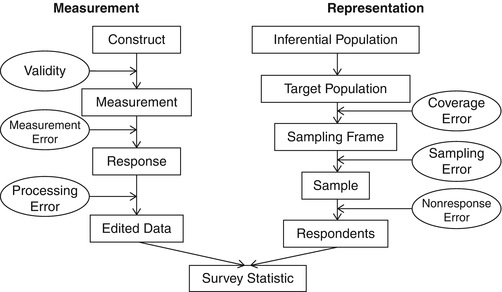
\includegraphics[width=0.8\linewidth]{total_survey_error} \caption{Source: [@Groves&Lyberg2010](https://doi.org/10.1093/poq/nfq065)}\label{fig:ext}
\end{figure}

The figure shows the survey process and the eventual sources of error.

\begin{quote}
The errors may be random or systematic
\end{quote}

In addition to substantial differences, different surveys are subject to differences sources of error.

\begin{quote}
Differences in systematic total survey error must then be reduced to 0 or kept equal across the groups we want to compare.
\end{quote}

A closer look to the \ref{ext} we can see a very simple distinction between Measurement and Representation. Both of these refer to goal of the survey to obtain the data as close to the ``true'' values as possible.

Systematic representation errors include:
- coverage error
- sampling error
- nonresponse

Systematic error in measurement include:
- validity
- processing
- measurement error

Measurement error includes: response error, interviewer-induced response effects, social desirability, methods effects, response styles.

\begin{quote}
Here we will focus on the Measurement side
\end{quote}

\hypertarget{bias-framework}{%
\section{Bias framework}\label{bias-framework}}

The classification of TSE is a close match to the Bias framework in the field of cross-cultural psychology.

In the field of cross‐cultural psychology Van de Vijver \& Leung (1997) distinguished ``construct'', ``item'', and ``method'' bias.

\begin{quote}
The bias framework is developed from the perspective of cross-cultural psychology and attempts to provide a comprehensive taxonomy of all systematic sources of error that can challenge the inferences drawn from cross-cultural studies (van de Vijver \& Leung, 1997, 2000; van de Vijver \& Poortinga, 1997; van de Vijver \& Tanzer, 2004).
\end{quote}

\hypertarget{three-types-of-bias-can-be-distinguished}{%
\subsection{Three types of bias can be distinguished}\label{three-types-of-bias-can-be-distinguished}}

\hypertarget{construct-bias}{%
\subsubsection{Construct Bias}\label{construct-bias}}

Construct bias is present if the underlying construct measured is not the same across cultures.

\begin{itemize}
\tightlist
\item
  It can occur if a construct is differently defined or only has a partial overlap across cultural groups.
\end{itemize}

Example:

\begin{quote}
Varying definitions of happiness in Western and East Asian cultures (Uchida, Norasakkunkit, \& Kitayama, 2004). In Western cultures, happiness tends to be defined in terms of individual achievement, whereas in East Asian cultures happiness is defined in terms of interpersonal connectedness.
\end{quote}

\hypertarget{method-bias}{%
\subsubsection{Method Bias}\label{method-bias}}

\begin{itemize}
\item
  Sample Bias: is the incomparability of samples due to cross-cultural variations in characteristics, such as different educational levels, students versus the general population, and urban versus rural residents
\item
  Instrument bias: involves systematic errors derived from instrument characteristics such as self-report bias in Likert-type scale measures. The systematic tendency of respondents to endorse certain response options on some basis other than the target construct (i.e., response styles) may affect the validity of cross- cultural comparisons (van Herk, Poortinga, \& Verhallen, 2004).
\item
  Administration Bias: stems from administration conditions (e.g., data collection modes, group versus individual assessment), ambiguous instructions, interaction between administrators and respondents (e.g., halo effects), and communication problems (e.g., language differences, taboo topic).
\end{itemize}

\hypertarget{item-bias}{%
\subsubsection{Item Bias}\label{item-bias}}

\begin{itemize}
\item
  Occurs when an item has a different meaning across cultures. An item of a scale is biased if persons with the same target trait level, but coming from different cultures, are not equally likely to endorse the item (van de Vijver \& Leung, 1997; van de Vijver, 2013).
\item
  Item bias can arise from poor translation, inapplicability of item contents in different cultures, or from items that trigger additional traits or have words with ambiguous connotations.
\end{itemize}

\hypertarget{preventing-comparability-problems-in-survey-research}{%
\chapter{Preventing comparability problems in survey research}\label{preventing-comparability-problems-in-survey-research}}

Here is a review of existing methods.

\hypertarget{measurement-invariance}{%
\chapter{Measurement Invariance}\label{measurement-invariance}}

The measurement invariance framework addresses the statistical implications of the bias framework and defines conditions that have to be fulfilled before inferences can be drawn about comparative conclusions dealing with constructs or scores in cross-cultural studies.

\begin{itemize}
\item
  Comparisons can only be made if the people in the different countries/cultures react similarly about the questions asked.
\item
  The measures should be ``functionally equivalent'' / the response models should be invariant across countries
\end{itemize}

Formal definition of invariance:

\begin{quote}
``whether or not, under different conditions of observing and studying phenomena, measurement operations yield measures of the same attribute'' (Horn \& McArdle, 1992, p.~117).
\end{quote}

\hypertarget{invariance-levels}{%
\section{Invariance Levels}\label{invariance-levels}}

Most research focus on 3 levels of invariance (some authors consider there are actually more\ldots)

\begin{itemize}
\item
  Configural Invariance (structural equivalence): model holds for all the groups
\item
  Metric Invariance (measurement unit equivalence): besides configural invariance, the slopes are the same in all the countries studied
\item
  Scalar Invariance (Full score equivalence): besides metric invariance, the intercepts are the same across all countries being compared.
\end{itemize}

\hypertarget{graphing-measurement-invariance}{%
\subsection{Graphing Measurement invariance}\label{graphing-measurement-invariance}}

\hypertarget{response-function}{%
\subsubsection{Response Function}\label{response-function}}

\begin{figure}
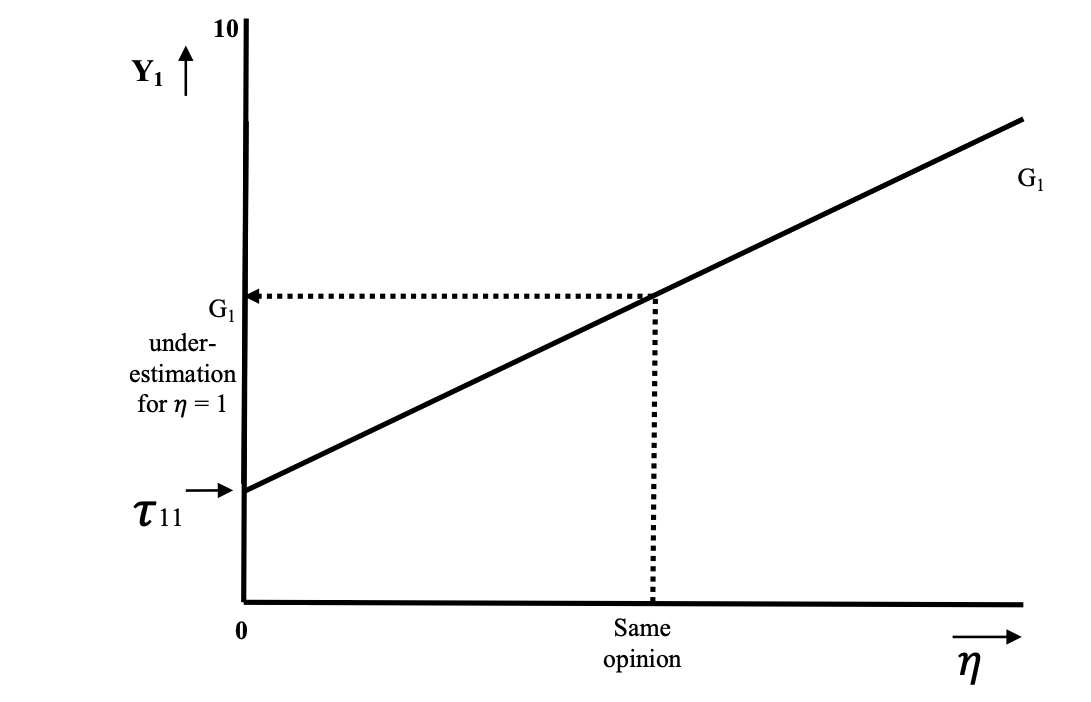
\includegraphics[width=0.8\linewidth]{response_function} \caption{Source: Adapted from Wicherts & Dolan}\label{fig:response}
\end{figure}

\hypertarget{metric-invariance}{%
\subsubsection{Metric Invariance}\label{metric-invariance}}

\begin{figure}
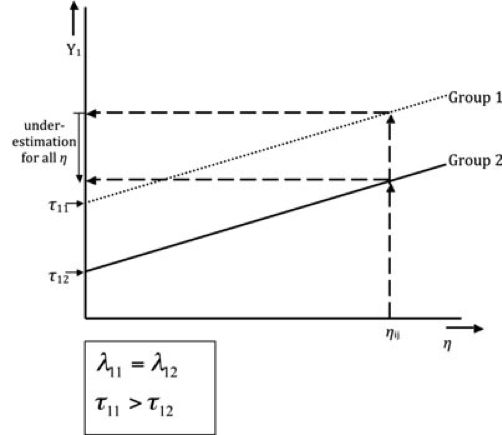
\includegraphics[width=0.8\linewidth]{Picture1} \caption{Source: Wicherts & Dolan, 2010}\label{fig:metric}
\end{figure}

\hypertarget{non-invariance}{%
\subsubsection{Non Invariance}\label{non-invariance}}

\begin{figure}
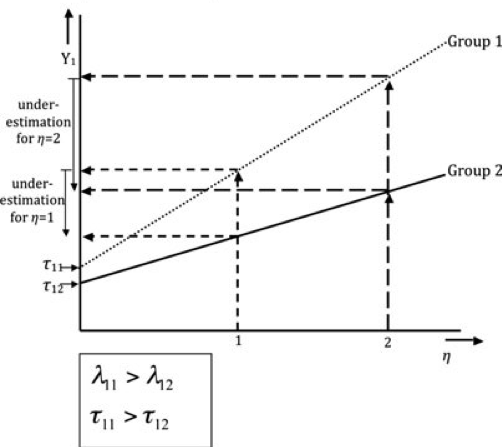
\includegraphics[width=0.8\linewidth]{Picture2} \caption{Source: Wicherts & Dolan, 2010}\label{fig:non}
\end{figure}

\hypertarget{metric-scalar-invariance}{%
\subsubsection{Metric \& Scalar Invariance}\label{metric-scalar-invariance}}

\begin{figure}
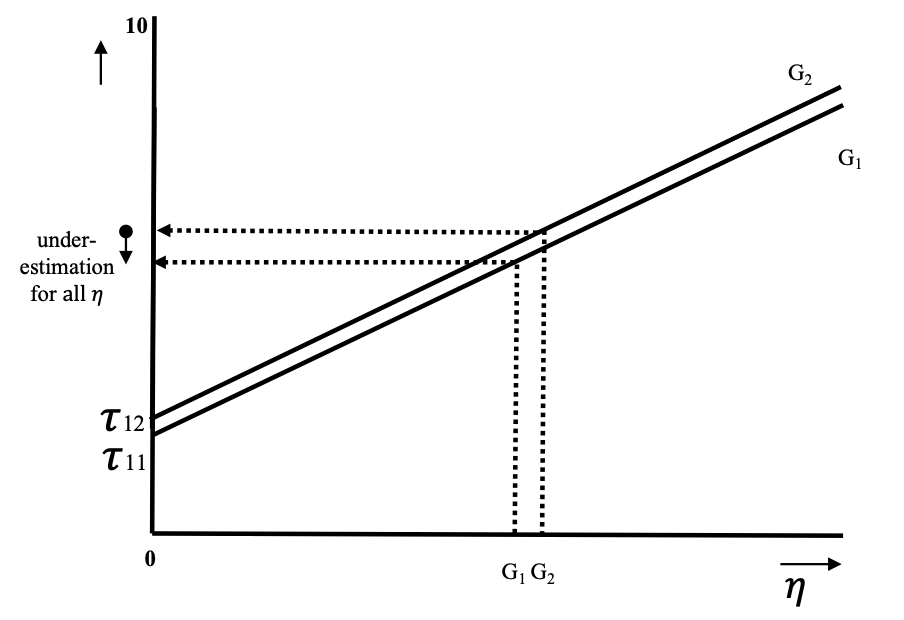
\includegraphics[width=0.8\linewidth]{metric_scalar} \caption{Source: Wicherts & Dolan, 2010}(\#fig:metric&scalar)
\end{figure}

\hypertarget{levels-of-invariance}{%
\section{Levels of Invariance}\label{levels-of-invariance}}

\begin{longtable}[]{@{}lrr@{}}
\toprule
Level of Invariance & Definition & Implication for group comparisons\tabularnewline
\midrule
\endhead
Configural & Same measurement model & Baseline model\tabularnewline
Metric & Identical factor loadings & relationships / correlations\tabularnewline
Scalar & Small intercept differences & Latent factor means\tabularnewline
\bottomrule
\end{longtable}

\hypertarget{how-to-test-for-measurement-invariance}{%
\section{How to test for measurement invariance?}\label{how-to-test-for-measurement-invariance}}

Factor Analysis

\begin{itemize}
\item
  Exploratory factor analysis (EFA) and comparing the structures across group (configuration of relations between construct and observed indicators)
\item
  Confirmatory factor analysis (CFA) and testing the invariance of the parameters = several steps(complete invariance of all is not always needed!)
\end{itemize}

\begin{center}\rule{0.5\linewidth}{0.5pt}\end{center}

\hypertarget{exploratory-factor-analysis}{%
\subsection{Exploratory Factor Analysis}\label{exploratory-factor-analysis}}

Exploratory factor analysis (EFA) is a multivariate statistical technique to model the covariance structure of the observed variables by three sets of parameters: (a) factor loadings associated with latent (i.e., unobserved) variables called factors, (b) residual variances called unique variances, and (c) factor correlations. EFA aims at explaining the relationship of many observed variables by a relatively small number of factors.

\begin{figure}
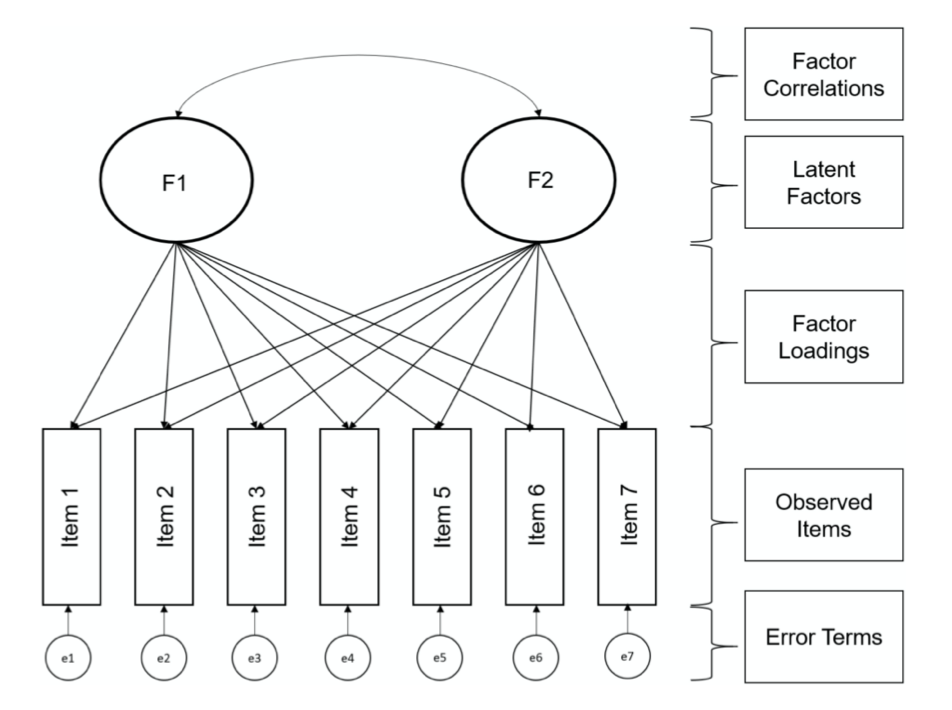
\includegraphics[width=0.8\linewidth]{expfactanal} \caption{Source: Wicherts & Dolan, 2010}\label{fig:factor}
\end{figure}

\hypertarget{confirmatory-factor-analysis}{%
\subsection{Confirmatory Factor Analysis}\label{confirmatory-factor-analysis}}

CFA focuses on modeling the relationship between manifest (i.e., observed) indicators and underlying latent variables (factors). CFA is a special case of structural equation modeling (SEM) in which relationships among latent variables are modeled as covariances/correlations rather than as structural relationships (i.e., regressions). CFA can also be distinguished from exploratory factor analysis (EFA) in that CFA requires researchers to explicitly specify all characteristics of the hypothesized measurement model (e.g., the number of factors, pattern of indicator- factor relationships) to be examined whereas EFA is more data-driven.

\begin{figure}
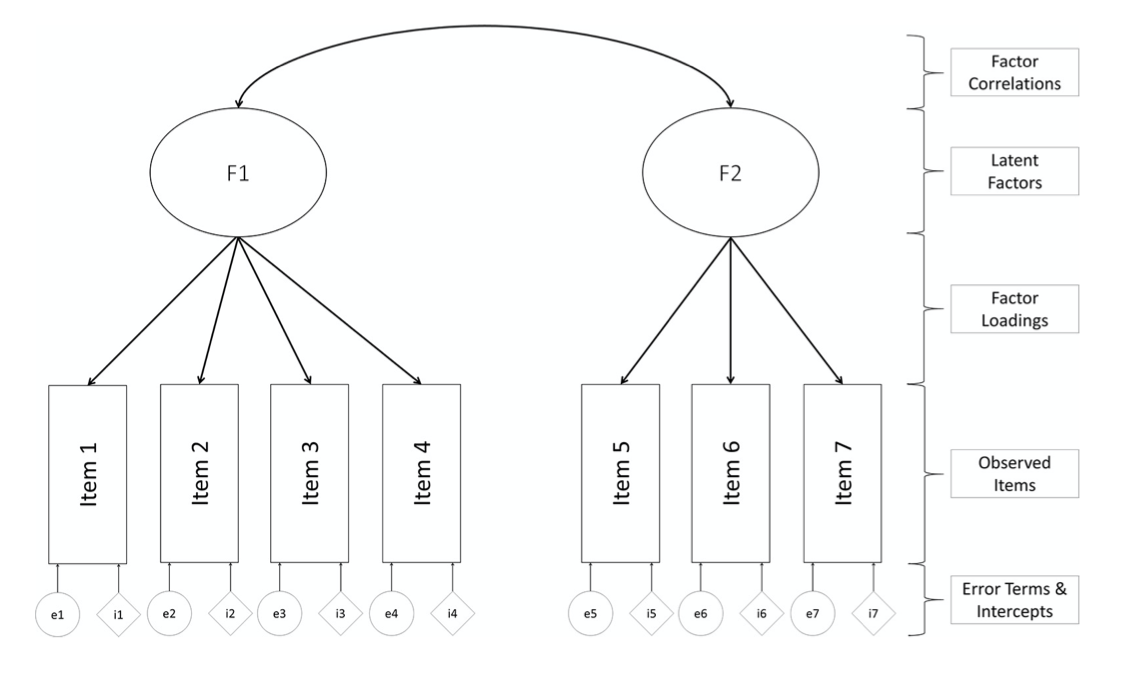
\includegraphics[width=0.8\linewidth]{confactor} \caption{Source: Wicherts & Dolan, 2010}\label{fig:cfa}
\end{figure}

For more information about confirmatory factor analysis see: \href{https://www.guilford.com/books/Confirmatory-Factor-Analysis-for-Applied-Research/Timothy-Brown/9781462515363}{Brown, T. A., Confirmatory Factor Analysis for Applied Research, Guilford Press}

\hypertarget{multi-group-confirmatory-factor-analysis---mgcfa}{%
\section{Multi-Group Confirmatory Factor Analysis - MGCFA}\label{multi-group-confirmatory-factor-analysis---mgcfa}}

\begin{itemize}
\item
  We can test whether a theoretical model fits several groups simultaneously
\item
  With a single model, we see how well it fits the data from all groups
\item
  How? Because we constrain parameters to be equal across groups
\item
  MGCFA invariance testing model in practice is testing an hypothesis of whether a given theoretical model fits well to the data across the groups.
\item
  Depending on what parameters we constraint to be equal across groups, we test one or another level of invariance
\end{itemize}

\begin{figure}
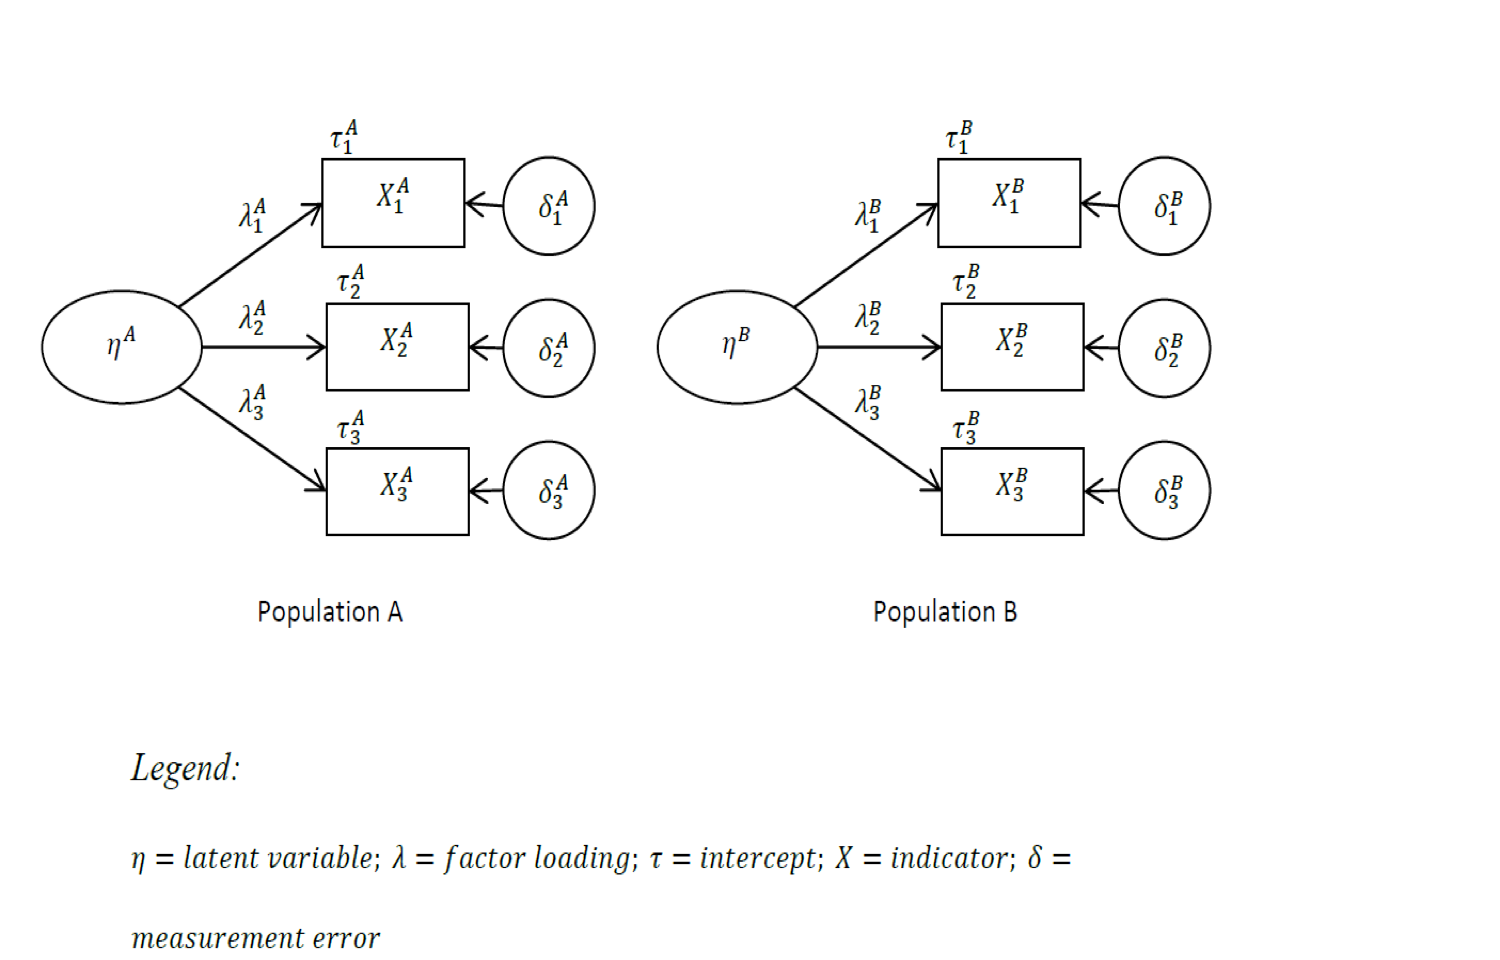
\includegraphics[width=0.8\linewidth]{multi_group} \caption{Source: Wicherts & Dolan, 2010}\label{fig:mgcfa}
\end{figure}

\hypertarget{alternative-measurement-invariance-testing-approaches-for-many-groups}{%
\chapter{Alternative measurement invariance testing approaches for many groups}\label{alternative-measurement-invariance-testing-approaches-for-many-groups}}

\hypertarget{exact-invariance-testing-alternative-approaches-to-mgcfa}{%
\subsection{Exact Invariance testing alternative approaches to MGCFA}\label{exact-invariance-testing-alternative-approaches-to-mgcfa}}

Multi-indicator Multiple Cause (MIMIC)

\begin{itemize}
\tightlist
\item
  MIMIC model permits both categorical and continuous individual difference variables (e.g., sex and age) but permits only a subset of the model parameters to vary as a function of these characteristic
\end{itemize}

See \href{https://journals.sagepub.com/doi/abs/10.1177/0013164411427395?journalCode=epma}{Kim et al., 2012}

Item Response Theory (IRT) Differential Item Functioning

\begin{itemize}
\tightlist
\item
  Aimed to categorical data
\end{itemize}

See \href{https://journals.sagepub.com/doi/10.1177/1094428114553062}{Tay et al., 2014}

\begin{center}\rule{0.5\linewidth}{0.5pt}\end{center}

\hypertarget{aproximate-invariance-a-conceptually-different-approach}{%
\subsection{Aproximate Invariance: a conceptually different approach}\label{aproximate-invariance-a-conceptually-different-approach}}

It is argued that a general measurement model using a CFA applies overly restrictive assumptions
that represent a theory-driven model (Brown, 2006, 2015; Marsh et al., 2012). Assumptions include that each measure loads on only one factor (e.g., assuming the absence of cross-loadings and residual correlations), the absence of effects from covariates, and the assumption of an exact invariant of the measures in MGCFA.

\begin{itemize}
\tightlist
\item
  In analysis of cross-national data, equality constraints tend to lead to the rejection of the tested model and often produce poor model fit statistics. Increasing the methodological sophistication and availability of statistical tools provide ways of quantifying uncertainty in the hypothesis through the estimation of possible values in the population rather than depending on only a single value for many populations.
\end{itemize}

\begin{figure}
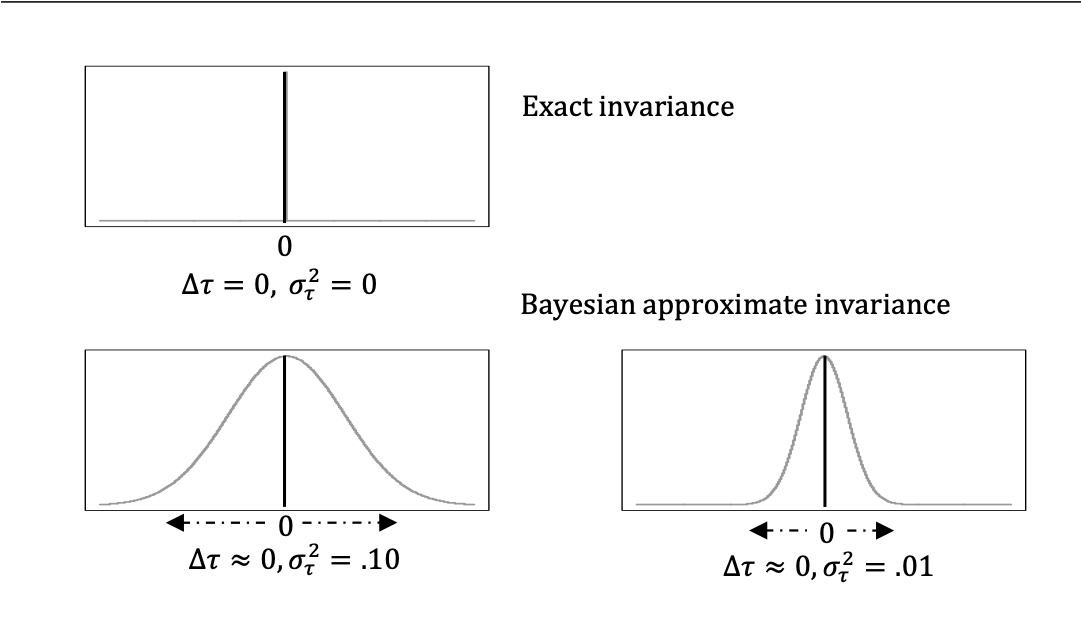
\includegraphics[width=0.8\linewidth]{approximate} \caption{Source: Wicherts & Dolan, 2010}\label{fig:approximate}
\end{figure}

Source \href{https://onlinelibrary.wiley.com/doi/abs/10.1002/9781118884997.ch40}{Desa et al., 2018}

\begin{itemize}
\item
  Alignment invariance \href{https://doi.org/10.1177/0049124117701488}{(Muthén \& Asparouhov, 2017)}
\item
  Bayesian SEM \href{https://onlinelibrary.wiley.com/doi/abs/10.1002/9781118884997.ch41}{(Lek et al.,2018)}
\item
  Mixture Models \href{https://www.researchgate.net/publication/338051963_Mixture_multigroup_factor_analysis_for_unraveling_factor_loading_non-_invariance_across_many_groups}{(Roover et al., 2019)}
\end{itemize}

\hypertarget{tutorial}{%
\chapter{Tutorial}\label{tutorial}}

Measurement invariance tutorial in R

\hypertarget{checklist-for-measurement-invariance-with-mgcfa}{%
\section{Checklist for measurement invariance with MGCFA}\label{checklist-for-measurement-invariance-with-mgcfa}}

\hypertarget{start-by-having-a-model}{%
\subsection{Start by having a model}\label{start-by-having-a-model}}

\begin{itemize}
\item
  Any statistical model is only as good as the theory it is built on.
\item
  Run CFA in each group to detect any large deviations.
\end{itemize}

\hypertarget{test-the-configural-model}{%
\subsection{Test the configural model}\label{test-the-configural-model}}

\begin{itemize}
\item
  Run a MGCFA without cross group equality constraints
\item
  The model should show a good fit.
\end{itemize}

\begin{quote}
There are two approaches of model identification: marker indicator or reference group
\href{https://www.tandfonline.com/doi/abs/10.1207/s15328007sem1301_3}{(see Little et al., 2006)}
\end{quote}

\hypertarget{test-the-metric-model}{%
\subsection{Test the metric model}\label{test-the-metric-model}}

\begin{itemize}
\item
  Fix the factor loadings to be equal across groups
\item
  Compare the model fit to the configural model
\end{itemize}

\hypertarget{test-the-scalar-model}{%
\subsection{Test the scalar model}\label{test-the-scalar-model}}

\begin{itemize}
\item
  In addition to the factor loadings, constrained the intercepts to be equal across groups
\item
  Compare the model fit to the metric model
\end{itemize}

\hypertarget{got-non-invariance-it-happens-often.}{%
\subsection{Got non-invariance? It happens often.}\label{got-non-invariance-it-happens-often.}}

\begin{itemize}
\item
  Several options:

  - exclude groups

  - remove items

  - distinguish several subgroups of countries
\end{itemize}

Still not getting invariance?

\begin{quote}
Conclude that the construct has different meaning across groups
\end{quote}

\begin{figure}
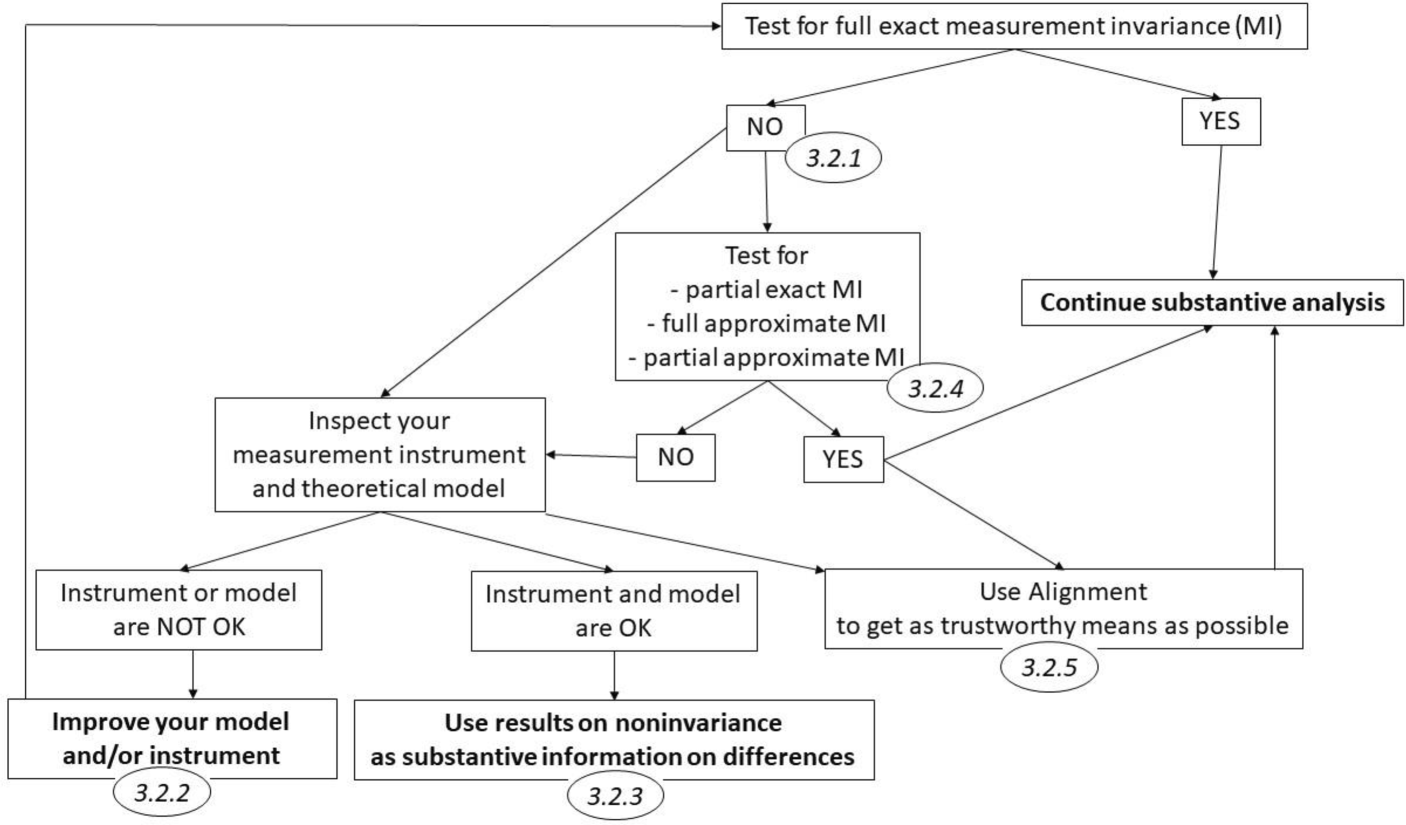
\includegraphics[width=0.8\linewidth]{decision_tree} \caption{Source: Wicherts & Dolan, 2010}\label{fig:tree}
\end{figure}

\hypertarget{mgcfa-in-r}{%
\section{MGCFA in R}\label{mgcfa-in-r}}

\hypertarget{how-to-run-a-mgcfa-in-r-the-overly-simple-way}{%
\subsection{How to Run a MGCFA in R (the overly simple way)}\label{how-to-run-a-mgcfa-in-r-the-overly-simple-way}}

Why R? Because it is free.

Alternatives:

\begin{itemize}
\item
  Mplus
\item
  Lisrel
\end{itemize}

\hypertarget{download-r-and-rstudio}{%
\subsection{Download R and RStudio}\label{download-r-and-rstudio}}

\begin{itemize}
\tightlist
\item
  \href{https://www.rstudio.com/products/rstudio/download/}{RStudio}
\item
  \href{https://cran.r-project.org}{R}
\end{itemize}

\hypertarget{install-lavaan-and-semtools}{%
\subsection{Install Lavaan and SemTools}\label{install-lavaan-and-semtools}}

\begin{itemize}
\tightlist
\item
  \href{https://cran.r-project.org/web/packages/lavaan/index.html}{Lavaan}
\item
  \href{https://cran.r-project.org/web/packages/semTools/index.html}{semTools}
\end{itemize}

\hypertarget{data-cleaning}{%
\subsection{Data cleaning}\label{data-cleaning}}

\begin{itemize}
\item
  Do whatever data wrangling necessary (missing values, etc)
\item
  Remember that you need a variable that identifies the group
\end{itemize}

\hypertarget{use-lavaan-language-to-formalize-the-model}{%
\subsection{Use Lavaan language to formalize the model}\label{use-lavaan-language-to-formalize-the-model}}

\begin{Shaded}
\begin{Highlighting}[]
\NormalTok{HS.model <-}\StringTok{ '  visual =~ x1 + x2 + x3}
\StringTok{              textual =~ x4 + x5 + x6}
\StringTok{              speed   =~ x7 + x8 + x9 '}
\NormalTok{fit <-}\StringTok{ }\KeywordTok{cfa}\NormalTok{(HS.model, }
           \DataTypeTok{data =}\NormalTok{ HolzingerSwineford1939, }
           \DataTypeTok{group =} \StringTok{"school"}\NormalTok{,}
           \DataTypeTok{group.equal =} \KeywordTok{c}\NormalTok{(}\StringTok{"loadings"}\NormalTok{))}
\KeywordTok{summary}\NormalTok{(fit)}
\end{Highlighting}
\end{Shaded}

\begin{verbatim}
lavaan (0.6-1) converged normally after  42 iterations

  Number of observations per group         
  Pasteur                                          156
  Grant-White                                      145

  Estimator                                         ML
  Model Fit Test Statistic                     124.044
  Degrees of freedom                                54
  P-value (Chi-square)                           0.000

Chi-square for each group:

  Pasteur                                       68.825
  Grant-White                                   55.219

Parameter Estimates:

  Information                                 Expected
  Information saturated (h1) model          Structured
  Standard Errors                             Standard


Group 1 [Pasteur]:

Latent Variables:
                   Estimate  Std.Err  z-value  P(>|z|)
  visual =~                                           
    x1                1.000                           
    x2      (.p2.)    0.599    0.100    5.979    0.000
    x3      (.p3.)    0.784    0.108    7.267    0.000
  textual =~                                          
    x4                1.000                           
    x5      (.p5.)    1.083    0.067   16.049    0.000
    x6      (.p6.)    0.912    0.058   15.785    0.000
  speed =~                                            
    x7                1.000                           
    x8      (.p8.)    1.201    0.155    7.738    0.000
    x9      (.p9.)    1.038    0.136    7.629    0.000

Covariances:
                   Estimate  Std.Err  z-value  P(>|z|)
  visual ~~                                           
    textual           0.416    0.097    4.271    0.000
    speed             0.169    0.064    2.643    0.008
  textual ~~                                          
    speed             0.176    0.061    2.882    0.004

Intercepts:
                   Estimate  Std.Err  z-value  P(>|z|)
   .x1                4.941    0.093   52.991    0.000
   .x2                5.984    0.100   60.096    0.000
   .x3                2.487    0.094   26.465    0.000
   .x4                2.823    0.093   30.371    0.000
   .x5                3.995    0.101   39.714    0.000
   .x6                1.922    0.081   23.711    0.000
   .x7                4.432    0.086   51.540    0.000
   .x8                5.563    0.078   71.087    0.000
   .x9                5.418    0.079   68.153    0.000
    visual            0.000                           
    textual           0.000                           
    speed             0.000                           

Variances:
                   Estimate  Std.Err  z-value  P(>|z|)
   .x1                0.551    0.137    4.010    0.000
   .x2                1.258    0.155    8.117    0.000
   .x3                0.882    0.128    6.884    0.000
   .x4                0.434    0.070    6.238    0.000
   .x5                0.508    0.082    6.229    0.000
   .x6                0.266    0.050    5.294    0.000
   .x7                0.849    0.114    7.468    0.000
   .x8                0.515    0.095    5.409    0.000
   .x9                0.658    0.096    6.865    0.000
    visual            0.805    0.171    4.714    0.000
    textual           0.913    0.137    6.651    0.000
    speed             0.305    0.078    3.920    0.000


Group 2 [Grant-White]:

Latent Variables:
                   Estimate  Std.Err  z-value  P(>|z|)
  visual =~                                           
    x1                1.000                           
    x2      (.p2.)    0.599    0.100    5.979    0.000
    x3      (.p3.)    0.784    0.108    7.267    0.000
  textual =~                                          
    x4                1.000                           
    x5      (.p5.)    1.083    0.067   16.049    0.000
    x6      (.p6.)    0.912    0.058   15.785    0.000
  speed =~                                            
    x7                1.000                           
    x8      (.p8.)    1.201    0.155    7.738    0.000
    x9      (.p9.)    1.038    0.136    7.629    0.000

Covariances:
                   Estimate  Std.Err  z-value  P(>|z|)
  visual ~~                                           
    textual           0.437    0.099    4.423    0.000
    speed             0.314    0.079    3.958    0.000
  textual ~~                                          
    speed             0.226    0.072    3.144    0.002

Intercepts:
                   Estimate  Std.Err  z-value  P(>|z|)
   .x1                4.930    0.097   50.763    0.000
   .x2                6.200    0.091   68.379    0.000
   .x3                1.996    0.085   23.455    0.000
   .x4                3.317    0.092   35.950    0.000
   .x5                4.712    0.100   47.173    0.000
   .x6                2.469    0.091   27.248    0.000
   .x7                3.921    0.086   45.555    0.000
   .x8                5.488    0.087   63.257    0.000
   .x9                5.327    0.085   62.786    0.000
    visual            0.000                           
    textual           0.000                           
    speed             0.000                           

Variances:
                   Estimate  Std.Err  z-value  P(>|z|)
   .x1                0.645    0.127    5.084    0.000
   .x2                0.933    0.121    7.732    0.000
   .x3                0.605    0.096    6.282    0.000
   .x4                0.329    0.062    5.279    0.000
   .x5                0.384    0.073    5.270    0.000
   .x6                0.437    0.067    6.576    0.000
   .x7                0.599    0.090    6.651    0.000
   .x8                0.406    0.089    4.541    0.000
   .x9                0.532    0.086    6.202    0.000
    visual            0.722    0.161    4.490    0.000
    textual           0.906    0.136    6.646    0.000
    speed             0.475    0.109    4.347    0.000

\end{verbatim}

Check out the \href{https://lavaan.ugent.be/tutorial/before.html}{lavaan tutorial}

\hypertarget{useful-shortcut-measurement-invariance-omnibus-testing}{%
\subsection{Useful shortcut: measurement invariance omnibus testing}\label{useful-shortcut-measurement-invariance-omnibus-testing}}

\begin{verbatim}
measurementInvariance(HS.model, 
                      data = HolzingerSwineford1939, 
                      group = "school")
\end{verbatim}

\begin{verbatim}
Measurement invariance models:

Model 1 : fit.configural
Model 2 : fit.loadings
Model 3 : fit.intercepts
Model 4 : fit.means

Chi Square Difference Test

               Df    AIC    BIC  Chisq Chisq diff Df diff Pr(>Chisq)    
fit.configural 48 7484.4 7706.8 115.85                                  
fit.loadings   54 7480.6 7680.8 124.04      8.192       6     0.2244    
fit.intercepts 60 7508.6 7686.6 164.10     40.059       6  4.435e-07 ***
fit.means      63 7543.1 7710.0 204.61     40.502       3  8.338e-09 ***
---
Signif. codes:  0 '***' 0.001 '**' 0.01 '*' 0.05 '.' 0.1 ' ' 1


Fit measures:

                 cfi rmsea cfi.delta rmsea.delta
fit.configural 0.923 0.097        NA          NA
fit.loadings   0.921 0.093     0.002       0.004
fit.intercepts 0.882 0.107     0.038       0.015
fit.means      0.840 0.122     0.042       0.015
\end{verbatim}

Terry Jorgensen \href{https://www.rdocumentation.org/packages/semTools/versions/0.4-14/topics/measurementInvariance}{measurementInvariance function}, within the semTools package is very handy

\hypertarget{conclusions}{%
\chapter{Conclusions}\label{conclusions}}

\begin{itemize}
\item
  Measurement invariance is important
\item
  Comparisons based on single questions without knowledge of the equivalence can be questioned
\item
  Adapt the measurement testing procedure to the model you want to test
\item
  Don't just think about measurement invariance when you get the data:
\end{itemize}

\begin{quote}
\textbf{Think about measurement invariance and actively include it during questionnaire design}
\end{quote}

\begin{itemize}
\item
  Remember MGCFA needs at least 3 indicators per latent variable to test for it.
\item
  Compare distributions and look for substantial deviations of the equality constraints over groups for slopes (factor loadings) and intercepts
\item
  Equivalente loadings (metric invariance) necessary for correlations, regressions
\item
  Equivalente intercepts (scalar invariance) necessary for comparing latent means
\item
  Comparing means and relationships between latent variables across countries does not have to require perfect invariance.
\item
  Using latent variables is a more flexible approach than employing composite scores.
\end{itemize}

\hypertarget{further-reading}{%
\chapter{Further Reading}\label{further-reading}}

\hypertarget{critical-issues-of-mgcfa-measurement-invariance}{%
\section{Critical Issues of MGCFA Measurement invariance}\label{critical-issues-of-mgcfa-measurement-invariance}}

\hypertarget{model-testing}{%
\subsection{Model testing}\label{model-testing}}

Quality of the model is the similarity of estimated parameters to the true population parameters (assuming the model is correct). However, cannot really observe this directly

\begin{itemize}
\tightlist
\item
  Model fit is the testing procedure and indicates the similarity between observed variance-covariance matrix and the variance-covariance matrix predicted by model.
\end{itemize}

Two testing approaches

\begin{itemize}
\tightlist
\item
  Global Fit indices: The most popular global fit measure is the χ2 test, but there are also many other fit indices that have been developed, such as the root mean squared error of approximation (RMSEA) or the comparative fit index (CFI). \href{https://www.tandfonline.com/doi/abs/10.1080/10705510701301834}{Chen (2007)} proposes that a change of larger than 0.01 in CFI is an indication of nonequivalence.
\end{itemize}

\begin{quote}
Most commonly used: chi-square, CFI, TLI, RMSEA, SRMR (all available by request in lavaan).
\end{quote}

\begin{itemize}
\tightlist
\item
  Local Fit indices: \href{https://www.tandfonline.com/doi/abs/10.1080/10705510903203433}{Saris et al.~(2009)} argue that global fit measures are never sufficient and that researchers should test the local fit of their models, that is, they should look at the parameter level and test if each of the parameters in the model is or not misspecified. Local fit testing tells whether there are misspecifications in the model using the modification indices (an estimate of the amount by which the χ2 would be reduced if a single parameter restriction was to be removed from the model), the power of the test (which is the complement of type II error, i.e., of wrongly failing to reject the null hypothesis), and when necessary the expected parameter changes (an approximation to the value of the parameter if it was not constrained).
\end{itemize}

\begin{quote}
Local fit testing: in R's semTools package \href{https://rdrr.io/cran/semTools/man/miPowerFit.html}{(miPowerFit)}; in Mplus \href{https://daob.nl/software/}{Jrule for Mplus}
\end{quote}

\begin{itemize}
\item
  Fit indices are not like R\textsuperscript{2}
\item
  High model fit does not guarantee theoretical soundness of the model. There are usually many models that have similarly good fit to the data, so you found only one of them.
\end{itemize}

\begin{center}\rule{0.5\linewidth}{0.5pt}\end{center}

\hypertarget{correction-for-measurement-error-in-invariance-testing}{%
\subsection{Correction for measurement error in invariance testing}\label{correction-for-measurement-error-in-invariance-testing}}

Without correction for measurement errors, we run the risk of giving explanations for differences between countries on substantive grounds that could be due to differences in measurement quality of the instruments.

\begin{itemize}
\item
  The problem with this approach is that the needed information is seldom available: quality estimates
\item
  The information about the quality can be derived from external sources such as MTMM experiments or SQP predictions.
\end{itemize}

\begin{quote}
Pirralha \& Weber (forthcoming) suggest to test on cognitive equivalence i.e.~invariance after correction for measurement errors.
\end{quote}

\begin{figure}
\centering
\includegraphics{corrected.tiff}
\caption{Measurement invariance testing after correction for measurement error}
\end{figure}

\begin{center}\rule{0.5\linewidth}{0.5pt}\end{center}

\hypertarget{sample-size-model-characteristics}{%
\subsection{Sample size \& Model Characteristics}\label{sample-size-model-characteristics}}

\begin{itemize}
\item
  Sample size cannot be too small.
\item
  Number of items per scale is very important. Large simulation study by \href{https://www.tandfonline.com/doi/abs/10.1080/10705511.2018.1561293}{Pokropek, Davidov \& Schmidt (2019)} shows that model characteristics such as number of items per scale is at least as important as invariance testing procedure
\item
  Take into account the nature of the observed items (ordinal, continuous, nominal, dichotomous)
\end{itemize}

\hypertarget{additional-resources}{%
\section{Additional resources}\label{additional-resources}}

\begin{itemize}
\item
  Highly reccomended: listen to the \href{https://quantitudethepodcast.org/listen/}{Quantitude Podcast} episode 12
\item
  Measurement Invariance checklists and tutorials:

  \begin{itemize}
  \tightlist
  \item
    \href{https://www.tandfonline.com/doi/abs/10.1080/17405629.2012.686740}{van de Schoot, Lugtig \& Hox, 2012}
  \item
    \href{https://www.frontiersin.org/articles/10.3389/fpsyg.2019.01507/full}{Fischer \& Karl, 2019}
  \item
    \href{https://lavaan.ugent.be/tutorial/groups.html}{Lavaan Measurement Invariance tutorial}
  \item
    Maksim Rudnev's \href{https://maksimrudnev.com/2019/05/01/alignment-tutorial/}{Alignment Invariance testing tutorial}
  \end{itemize}
\end{itemize}

  \bibliography{book.bib,packages.bib}

\end{document}
